\begin{center}
\vspace{-0.5cm}
\tikzstyle{block} = [rectangle, draw, fill=blue!20,
text width=1.5cm, text centered, rounded corners, minimum height=1.5cm]	
\def\rectDiv#1#2#3#4#5{%#columns, #rows, rectangle start, rectangle end, list of elements to fill
\draw #3 rectangle #4;
\path #3;
\pgfgetlastxy{\firstx}{\firsty}
\path #4;
\pgfgetlastxy{\secondx}{\secondy}
\pgfmathsetlengthmacro{\xdiff}{\secondx-\firstx}
\pgfmathsetlengthmacro{\ydiff}{\secondy-\firsty}
\pgfmathsetlengthmacro{\myxstep}{\xdiff/#1}
\pgfmathsetlengthmacro{\myystep}{\ydiff/#2}
\foreach \x in {1,...,#1}{
	\draw ($#3 +\x*(\myxstep,0)$) -- ($#3 +(0,\ydiff) +\x*(\myxstep,0)$);
}
\foreach \y in {1,...,#2}{
	\draw ($#3 +\y*(0,\myystep)$) -- ($#3 +(\xdiff,0) +\y*(0,\myystep)$);
}
\foreach \i/\j in {#5}{
	\path[fill=darkgreen!20,draw] ($#3 + (\i*\myxstep,\j*\myystep)$) rectangle ($#3 + (\i*\myxstep,\j*\myystep) + (\myxstep,\myystep)$);
}
}
\def\rectDivred#1#2#3#4#5{%#columns, #rows, rectangle start, rectangle end, list of elements to fill
\draw #3 rectangle #4;
\path #3;
\pgfgetlastxy{\firstx}{\firsty}
\path #4;
\pgfgetlastxy{\secondx}{\secondy}
\pgfmathsetlengthmacro{\xdiff}{\secondx-\firstx}
\pgfmathsetlengthmacro{\ydiff}{\secondy-\firsty}
\pgfmathsetlengthmacro{\myxstep}{\xdiff/#1}
\pgfmathsetlengthmacro{\myystep}{\ydiff/#2}
\foreach \x in {1,...,#1}{
	\draw ($#3 +\x*(\myxstep,0)$) -- ($#3 +(0,\ydiff) +\x*(\myxstep,0)$);
}
\foreach \y in {1,...,#2}{
	\draw ($#3 +\y*(0,\myystep)$) -- ($#3 +(\xdiff,0) +\y*(0,\myystep)$);
}
\foreach \i/\j in {#5}{
	\path[fill=red!20,draw] ($#3 + (\i*\myxstep,\j*\myystep)$) rectangle ($#3 + (\i*\myxstep,\j*\myystep) + (\myxstep,\myystep)$);
}
}
\tikzset{tbox/.style={draw, text badly centered, very thick, black, rectangle, inner sep=0, minimum width = 2.0 cm, minimum height = 1.0 cm}}
\begin{tikzpicture}[x=1cm,y=1cm]
%\pgfresetboundingbox
\draw[use as bounding box, anchor = north west,draw=none] (-2,-3.5) rectangle (9.5,3.5);
\clip (-2,-3.25) rectangle (9.0,3.25);
\node (ds) at (0,0){};
\node (dsy) at (0,4){};
\node (dsx) at (4,0){};
\def \cssize {1.0 cm}
\def \psize {1.15 cm}
\def\circledarrow#1#2#3{ % #1 Style, #2 Center, #3 Radius
	\draw[#1,->] (#2) +(80:#3) arc(80:-260:#3);}
%% now the flow chart
%% define coordinate grid 
\def \xfarleft {1}
\def \xleft {2.5}
\def \xmid {5.25}
\def \xright {8}
\def \ytop {2.75}
\def \ymid {0.5}
\def \ybot {-2.5}
\def \yphasetwo {-2.0}
\def \xlabeloffset {0.05}
\def \ylabeloffset {0.15}

%% title/step tracking
\node[anchor=north west] (title) at (4,3.3) {\large 
	\only<1>{\textbf{1. Collect data ($X,y$)}}
	\only<2>{\textbf{2. Featurize}}
	\only<3-4>{\textbf{3. Partition data}}
	\only<5-10>{\textbf{4. Learning phase}}
	\only<11->{\textbf{5. Testing phase}}
};


%% molecules
\only<1-2>{
{\node[circle,draw, thick, minimum width =\cssize,path picture={\node at (path picture bounding box.center){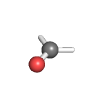
\includegraphics[width= \psize]{satistical_learning/images/m1}}; }] (m1) at (1,2.75){};}
{\node[circle,draw, thick, minimum width = \cssize,path picture={\node at (path picture bounding box.center){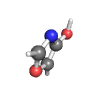
\includegraphics[width= \psize]{satistical_learning/images/m2}}; }] (m2) at (2,2.0){};}
{\node[circle,draw, thick, minimum width = \cssize,path picture={\node at (path picture bounding box.center){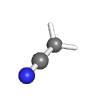
\includegraphics[width= \psize]{satistical_learning/images/m3}}; }] (m3) at (3,1.25){};}
{\node[circle,draw, thick, minimum width = \cssize,path picture={\node at (path picture bounding box.center){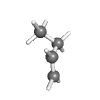
\includegraphics[width= \psize]{satistical_learning/images/m4}}; }] (m4) at (4,0.5){};}
{\node[circle,draw, thick, minimum width = \cssize,path picture={\node at (path picture bounding box.center){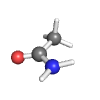
\includegraphics[width= \psize]{satistical_learning/images/m5}}; }] (m5) at (5,-0.25){};}
{\node[circle,draw, thick, minimum width = \cssize,path picture={\node at (path picture bounding box.center){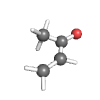
\includegraphics[width= \psize]{satistical_learning/images/m6}}; }] (m6) at (6,-1.0){};}
{\node[circle,draw, thick, minimum width = \cssize,path picture={\node at (path picture bounding box.center){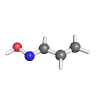
\includegraphics[width= \psize]{satistical_learning/images/m7}}; }] (m7) at (7,-1.75){};}
{\node[circle,draw, thick, minimum width = \cssize,path picture={\node at (path picture bounding box.center){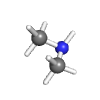
\includegraphics[width= \psize]{satistical_learning/images/m8}}; }] (m8) at (8,-2.5){};}
}


%% mol to vect mapping
\only<2>{
\foreach  \namey / \y in {m1/1.75,m2/1.25,m3/0.75,m4/0.25,m5/-0.25,m6/-0.75,m7/-1.25,m8/-1.75}{
	\visible<1->{\draw [black,thick,->] (\namey) -- (-1,\y) ;}}
\node[anchor=north west] (thislab) at (-1,-2.75) {convert to vectors, preprocess, scale -- not simple!};
}

%% rectangles
\visible<2>{\rectDivred{1}{8}{(-1.5,-2)}{(-1.0,2)}{};}
\visible<3>{\rectDivred{1}{8}{(-1.5,-2)}{(-1.0,2)}{0/0,0/1};}
\only<3>{
\node[rotate=90] (thislab) at (-1.75,0.5) {training data};
\node[rotate=90, red] (thislab) at (-1.75,-1.5) {test data};
}
\visible<4->{\rectDivred{1}{6}{(-1.5,0)}{(-1.0,3)}{};}
\visible<4->{\rectDivred{1}{2}{(-1.5,-3)}{(-1.0,-2)}{0/0,0/1};}
%% labels to blocks
\only<4>{
	\node[rotate=90] (thislab) at (-1.75,1.5) {training data};
	\node[rotate=90, red] (thislab) at (-1.75,-2.5) {test data};
}

%% train phase
\only<1-10>{
%% start learning proc with training data
\visible<5->{
	\node [tbox,minimum width=2.0 cm, text width = 2.0 cm] (traindata) at (\xfarleft,\ytop) {training data};
\node [] (traindatay) at (\xright,\ytop) {};
}
\only<5->{
	\path[draw,dashed] (-1,3) -- (traindata.north west);
	\path[draw,dashed] (-1,0) -- (traindata.south west);	
}

%% show model
\visible<6->{
	\node [tbox,minimum width=2.0 cm, text width = 2.0 cm] (model) at (\xleft,\ymid) {model};
	\draw [thick, black,->] (traindata.south) |-  (model.west);
	\node[anchor=west] (inputslab) at (\xfarleft + \xlabeloffset,0.5*\ymid + 0.5*\ytop)  {inputs, $X$};
}
\only<6-8>{
	\node[anchor=east] (paramslabtemp) at (\xleft - \xlabeloffset,0.5*\ymid + 0.5*\ybot)  {parameters, $W$};
	\draw [thick, black,->] ([yshift=-2cm]model.south) -- (model.south);
}
%% loss needs to be defined out of sequence for reference purposes
\visible<8->{
	\node [tbox,minimum width=2.0 cm, text width = 2.0 cm] (lossf) at (\xright,\ymid) {loss function};
	\draw [thick, black,->] (traindata.east) -- (traindatay.center) -- (lossf.north);
	\node[anchor=east] (labslab) at (\xright - \xlabeloffset,0.5*\ymid + 0.5*\ytop)  {labels, $y(X)$};
}
%% show parameter depedences , out of order to allow modelparams
\visible<9->{
	\node [tbox,minimum width=2.0 cm, text width = 2.0 cm] (modelparams) at (\xmid,\ybot) {update parameters};
	\node[anchor=east] (paramslab) at (\xleft - \xlabeloffset,0.5*\ymid + 0.5*\ybot)  {parameters, $W$};
	\draw [thick, black,->] (modelparams.west) -| (model.south);
	\node[anchor=east] (errorslab) at (\xright - \xlabeloffset,0.5*\ymid + 0.5*\ybot)  {loss, $\mathcal{L}$};
	\draw [thick, black,->] (lossf.south) |- (modelparams.east);
}

\only<8>{
\node[anchor=east] (errorslabtemp) at (\xright - \xlabeloffset,0.5*\ymid + 0.5*\ybot)  {loss, $\mathcal{L}$};
\draw [thick, black,->] (lossf.south) -- ([yshift=-2.cm]lossf.south);
}

%% show predictions
\visible<7->{
\node[anchor=south] (predslab) at (\xmid,\ymid + \ylabeloffset)  {predictions, $\hat{y}(X)$};
\draw [thick, black,->] (model.east) to node [midway,above,label={[label distance=0.15cm]90:}] {} (lossf.west);
}

%% repeat until converged label
\visible<10->{
\node[text width = 2.0cm,text badly centered] (text) at (\xmid,-0.75) {repeat until converged};
\circledarrow{thick, black}{text}{1cm};
}

}

%% testing phase

\only<11->{
%% start learning proc with training data
\node [tbox,minimum width=2.0 cm, text width = 2.0 cm,opacity=0.10] (traindata) at (\xfarleft,\ytop) {training data};
\node [] (traindatay) at (\xright,\ytop) {};
\path[draw,dashed,opacity=0.10] (-1,3) -- (traindata.north west);
\path[draw,dashed,opacity=0.10] (-1,0) -- (traindata.south west);	
\node [tbox,minimum width=2.0 cm, text width = 2.0 cm] (model) at (\xleft,\ymid) {model};
\draw [thick, black,->,opacity=0.10] (traindata.south) |-  (model.west);
\node[anchor=west,opacity=0.10] (inputslab) at (\xfarleft + \xlabeloffset,0.5*\ymid + 0.5*\ytop)  {inputs, $X$};


\node[anchor=west,blue] (paramslabtemp) at (\xleft + \xlabeloffset,0.5*\ymid + 0.5*\ybot)  {parameters, $W$};
\draw [thick, blue,->] ([yshift=-2cm]model.south) -- (model.south);

\node [tbox,minimum width=2.0 cm, text width = 2.0 cm,opacity=0.10] (lossf) at (\xright,\ymid) {loss function};
\draw [thick, black,->,opacity=0.10] (traindata.east) -- (traindatay.center) -- (lossf.north);
\node[anchor=east,opacity=0.10] (labslab) at (\xright - \xlabeloffset,0.5*\ymid + 0.5*\ytop)  {labels, $y(X)$};


\node [tbox,minimum width=2.0 cm, text width = 2.0 cm,opacity=0.10] (modelparams) at (\xmid,\ybot) {update parameters};

\draw [thick, black,->,opacity=0.10] (modelparams.west) -| (model.south);
\node[anchor=east,opacity=0.10] (errorslab) at (\xright - \xlabeloffset,0.5*\ymid + 0.5*\ybot)  {loss, $\mathcal{L}$};
\draw [thick, black,->,opacity=0.10] (lossf.south) |- (modelparams.east);
\node[anchor=east,opacity=0.10] (errorslabtemp) at (\xright - \xlabeloffset,0.5*\ymid + 0.5*\ybot)  {loss, $\mathcal{L}$};
\draw [thick, black,->,opacity=0.10] (lossf.south) -- ([yshift=-2.cm]lossf.south);

\node[anchor=south,opacity=0.10] (predslab) at (\xmid,\ymid + \ylabeloffset)  {predictions, $\hat{y}(X)$};
\draw [thick, black,->,opacity=0.10] (model.east) to node [midway,above,label={[label distance=0.15cm]90:}] {} (lossf.west);


}


\visible<12->{
\node [tbox,minimum width=2.0 cm, text width = 2.0 cm] (testdata) at (\xfarleft,\yphasetwo) {test data};}
\only<12->{
	\path[draw,dashed,red] (-1,-2) -- (testdata.north west);
	\path[draw,dashed,red] (-1,-3) -- (testdata.south west);	
}

\visible<13->{
\draw [thick, black,->] (testdata.north) |-  (model.west);
\node[anchor=east] (testxlab) at (\xfarleft-\xlabeloffset,0.5*\yphasetwo + 0.5*\ymid)  {inputs, $X^*$};
\node[anchor=north] (testpredslab) at (\xmid,\ymid - \ylabeloffset)  {predictions, $\hat{y}(X^*)$};
}
\only<13>{
\draw [thick, black,->] (model.east) --  ([xshift=2cm]model.east) ;
}

\visible<14->{
\node [tbox,minimum width=2.0 cm, text width = 2.0 cm] (evalf) at (\xright,\yphasetwo) {evaluation};
\draw [thick, black,->] (model.east) -|  (evalf.north);

}

\end{tikzpicture}
\end{center}